\documentclass[14pt]{extarticle}
\usepackage[utf8]{inputenc}
\usepackage{amsmath}
\usepackage{amsfonts}
\usepackage{graphicx}
\usepackage{setspace}
\usepackage{geometry}
\usepackage{enumitem}
\usepackage{amssymb}
\usepackage{xcolor}
\usepackage{mathtools}
\usepackage{float}
\usepackage{listings}

% 调整字符间距的命令
\makeatletter
\newcommand\fixspacing{\fontdimen2\font=0.3em} % 0.3em 可以调整为更小的值
\makeatother

\lstset{
    backgroundcolor=\color{lightgray},      % 灰色背景
    basicstyle=\ttfamily\normalsize\fixspacing, % 正常字体大小并且字符间距调整
    frame=single,                          % 给代码加框
    columns=flexible,                      % 允许字符宽度根据字符间距调整
    breaklines=false,                      % 不自动换行
    showspaces=false,                      % 不显示空格
    showstringspaces=false,                % 不显示字符串中的空格
    tabsize=2,                             % Tab 的宽度
    numbers=none,                          % 不显示行号
    xleftmargin=0pt,                       % 确保左边没有额外的内边距
    framexleftmargin=1pt,                  % 消除框与代码左边的距离
    framesep=0pt,                          % 代码与框线之间的距离为 0
    aboveskip=0pt,                         % 取消上方的空隙
    belowskip=0pt                          % 取消下方的空隙
}

\geometry{
    top=1in,
    bottom=1in,
    left=1in,
    right=1in,
    headheight=14pt,
    headsep=25pt,
    footskip=30pt
}

\title{Bayes Theorem}
\author{Yana Jin}
\date{Wednesday, 16th September 2024}

\onehalfspacing

\newcommand{\coverpage}{%
    \begin{titlepage}
        \centering
        
\includegraphics[width=1\textwidth]{cover.png}
    \end{titlepage}
}

\begin{document}

\coverpage

\newpage



\section*{Confidence Intervals and Power}

\subsection*{CIs via hypothesis tests}

\textbf{One-sample tests}

Recall:
\( H_0: E(Y) = \mu_0 \) is \textcolor{blue}{rejected} if:
\[
\sqrt{n} | \frac{(\bar{y} - \mu_0)}{s} | \geq t_{1-\alpha/2} \textcolor{red}{ \left( t_{n-1} \right)}
\]
\( H_0: E(Y) = \mu_0 \) is \textcolor{blue}{not rejected} if:
\[
\sqrt{n} | \frac{(\bar{y} - \mu_0)}{s} | \leq t_{1-\alpha/2} \textcolor{red}{ \left( t_{n-1} \right)}
\]
\[
\Rightarrow | \bar{y} - \mu_0 | \leq \frac{s}{\sqrt{n}} \times t_{1-\alpha/2}
\]
\[
\Rightarrow \bar{y} - \frac{s}{\sqrt{n}} t_{1-\alpha/2} \leq \mu_0 \leq \bar{y} + \frac{s}{\sqrt{n}} t_{1-\alpha/2}
\]
If \(\mu_0\) satisfies the last line, then it is in the "acceptance / non-rejection" region.

\noindent If not, it is in the rejection region.
\[
\Rightarrow \text{"plausible"} \text{ values of } \mu \text{ are in the interval}
\]
\[
\bar{y} \pm \frac{s}{\sqrt{n}} t_{1-\alpha/2}
\]
We call this a \(100 \times (1-\alpha)\%\) confidence interval (CI) for \(\mu\). 
\[
\textcolor{blue}{\left[ \text{contains only those values of } \mu \text{ not rejected by this level-}\alpha \text{ test} \right]}
\]


\subsection*{Main property of CI}
\textbf{Suppose you } 1) \text{ gather data} \quad  and 2) compute $ 100 \times (1 - \alpha ) \% $ CI

\noindent \textbf{Also assume } $H_0: E(Y) = \mu_0$ \text{ is true.}

\noindent \text{What is the probability that } $\mu_0$ \text{ will be in a to-be-sampled (} \textcolor{blue}{\text{random}} \text{) interval?}
\[
P(\mu_0 \text{ in interval } \mid E(Y) = \mu_0)
\]
\[
= 1 - P(\mu_0 \text{ not in interval } \mid E(Y) = \mu_0)
\]
\[
= 1 - P(\text{reject } H_0 \mid E(Y) = \mu_0)
\]
\[
= 1 - P(\text{reject } H_0 \mid H_0 \text{ true})
\]
\[
= 1 - \alpha
\]
\((1 - \alpha)\) \text{ is called } \textcolor{blue}{\text{coverage probability}} \text{ of the interval.}

\vspace{0.5cm}
\textbf{Interpretation:}
\begin{itemize}
    \item \text{pre-experimental probability that the CI will cover the true value}
    \item \text{the large sample fraction of experiments in which the CI covers the true mean.}
\end{itemize}

\subsection*{CI for two sample test}

\textbf{Recall:} can construct a $95\%$ CI for $(\mu_B - \mu_A)$ by finding those null hypotheses that would not be rejected at $\alpha = 0.05$ level.

\noindent \textbf{Sampling model:}
\[
Y_{1A}, \dots, Y_{n_A A} \sim \text{i.i.d. } \mathcal{N}(\mu_A, \sigma^2)
\]
\[
Y_{1B}, \dots, Y_{n_B B} \sim \text{i.i.d. } \mathcal{N}(\mu_B, \sigma^2)
\]
\noindent Consider whether $\delta$ is a reasonable value for the difference in population means.
\[
H_0: \mu_B - \mu_A = \delta
\]
\[
H_1: \mu_B - \mu_A \neq \delta
\]
Under $H_0$:
\[
\frac{(\bar{Y}_B - \bar{Y}_A) - \delta}{s_p \sqrt{\frac{1}{n_A} + \frac{1}{n_B}}} \sim t_{n_A + n_B - 2}
\]
Thus $\delta$  is \textcolor{blue}{\text{accepted}} at level $\alpha$ if observed value
\[
\frac{|(\bar{y}_B - \bar{y}_A) - \delta|}{s_p \sqrt{\frac{1}{n_A} + \frac{1}{n_B}}} \leq t_c \quad
\textcolor{red}{\leftarrow \text{critical value}}
\]
\[
\Rightarrow (\bar{y}_B - \bar{y}_A) - s_p \sqrt{\frac{1}{n_A} + \frac{1}{n_B}} \leq \delta \leq (\bar{y}_B - \bar{y}_A) + s_p \sqrt{\frac{1}{n_A} + \frac{1}{n_B}}
\]
\[
\text{where} \quad
t_c = t_{1-\alpha/2, n_A + n_B - 2}
\]
\noindent \text{From earlier example:}
\begin{itemize}
    \item $\bar{y}_B - \bar{y}_A = 5.93$
    \item $s_p = 4.72, s_p \sqrt{\frac{1}{n_A} + \frac{1}{n_B}} = 2.72$
    \item $t_{.975, 10} = 2.23$
\end{itemize}

A $95\%$ confidence interval (CI) for $\mu_B - \mu_A$ is
\[
5.93 \pm 2.72 \times 2.23
\]
\[
5.93 \pm 6.07 = (-0.13, 11.99)
\]



\newpage
\section*{Power and Sample Size Determination}
\textbf{Consider}
\[
H_0: \mu_A = \mu_B
\]
\[
H_1: \mu_A \neq \mu_B
\]
Perform a level $\alpha$ test: reject $H_0$ if
\[
|t_{\text{obs}}| \geq t_{1-\alpha/2, n_A + n_B - 2}
\]
We know if $\alpha = 0.05$ :
\[
\Rightarrow P(\text{type I error} \mid H_0 \text{ true}) = P(\text{reject } H_0 \mid H_0 \text{ true}) = 0.05
\]
What about
\[
P(\text{type II error} \mid H_0 \text{ false}) ?
\]

\[
= P(\text{do not reject } H_0 \mid H_0 \text{ false})
\]

\[
= 1 - P(\text{reject } H_0 \mid H_0 \text{ false})
\]

\noindent \textcolor{blue}{Not a well-defined calculation since conditioning argument not clearly specified} \textcolor{red}{What is $H_0$ false?}

\noindent We need to refer to a \textcolor{blue}{specific} alternative hypothesis.
\[
1 - P(\text{type II error} \mid (\mu_B - \mu_A) = \delta)
\]
\[
= P(\text{reject } H_0 \mid (\mu_B - \mu_A) = \delta)
\]
\[
= \text{Power}(\delta)
\]
For two sample t-test:
\[
\Rightarrow P\left( |t(Y_A, Y_B)| \geq t_{1-\alpha/2, n_A+n_B-2} \mid \delta \right)
\]

\noindent $\therefore$ we need to know the distribution of our t-statistic under the specific alternative hypothesis.

\noindent We need to know the distribution of
\[
t(Y_A, Y_B) = \frac{\bar{Y}_B - \bar{Y}_A}{s_p \sqrt{\frac{1}{n_A} + \frac{1}{n_B}}} \text{ when } \mu_B - \mu_A = \delta
\]
Recall, we know if \(\mu_B - \mu_A = \delta\)
\[
\frac{(\bar{Y}_B - \bar{Y}_A) - \delta}{s_p \sqrt{\frac{1}{n_A} + \frac{1}{n_B}}} \sim t_{n_A + n_B - 2}
\]

but
\[
t(Y_A, Y_B) = \frac{(\bar{Y}_B - \bar{Y}_A) - \delta}{s_p \sqrt{\frac{1}{n_A} + \frac{1}{n_B}}} + \frac{\delta}{\textcolor{red}{s_p \sqrt{\frac{1}{n_A} + \frac{1}{n_B}}}}
\]

\textcolor{red}{\text{move t-statistic away from being centered at zero.}$\nearrow$}
\[\textcolor{blue}{\text{(amount depends on } s_p )}\]
\[
\Rightarrow t(Y_A, Y_B) \sim t^*_{n_A + n_B - 2} \left( \frac{\delta}{\textcolor{red}{\sigma \sqrt{\frac{1}{n_A} + \frac{1}{n_B}}}} \right)
\]
\[
\textcolor{red}{\sigma \text{ is non-centrality parameter } \uparrow}
\]

\subsection*{The Non-central t-distribution}
A non-central t-distributed random variable is represented as
\[
T = \frac{Z + \delta}{\sqrt{X / \nu}}
\]
\[
\text{where }\quad
\textcolor{red}{\delta \text{ is a constant, } \quad Z \sim N(0, 1), \quad X \sim \chi^2_\nu}
\]
\[\textcolor{blue}{\delta \text{ is "non-centrality parameter"}}\]

\textbf{Example}
\begin{figure}[h]
    \centering
    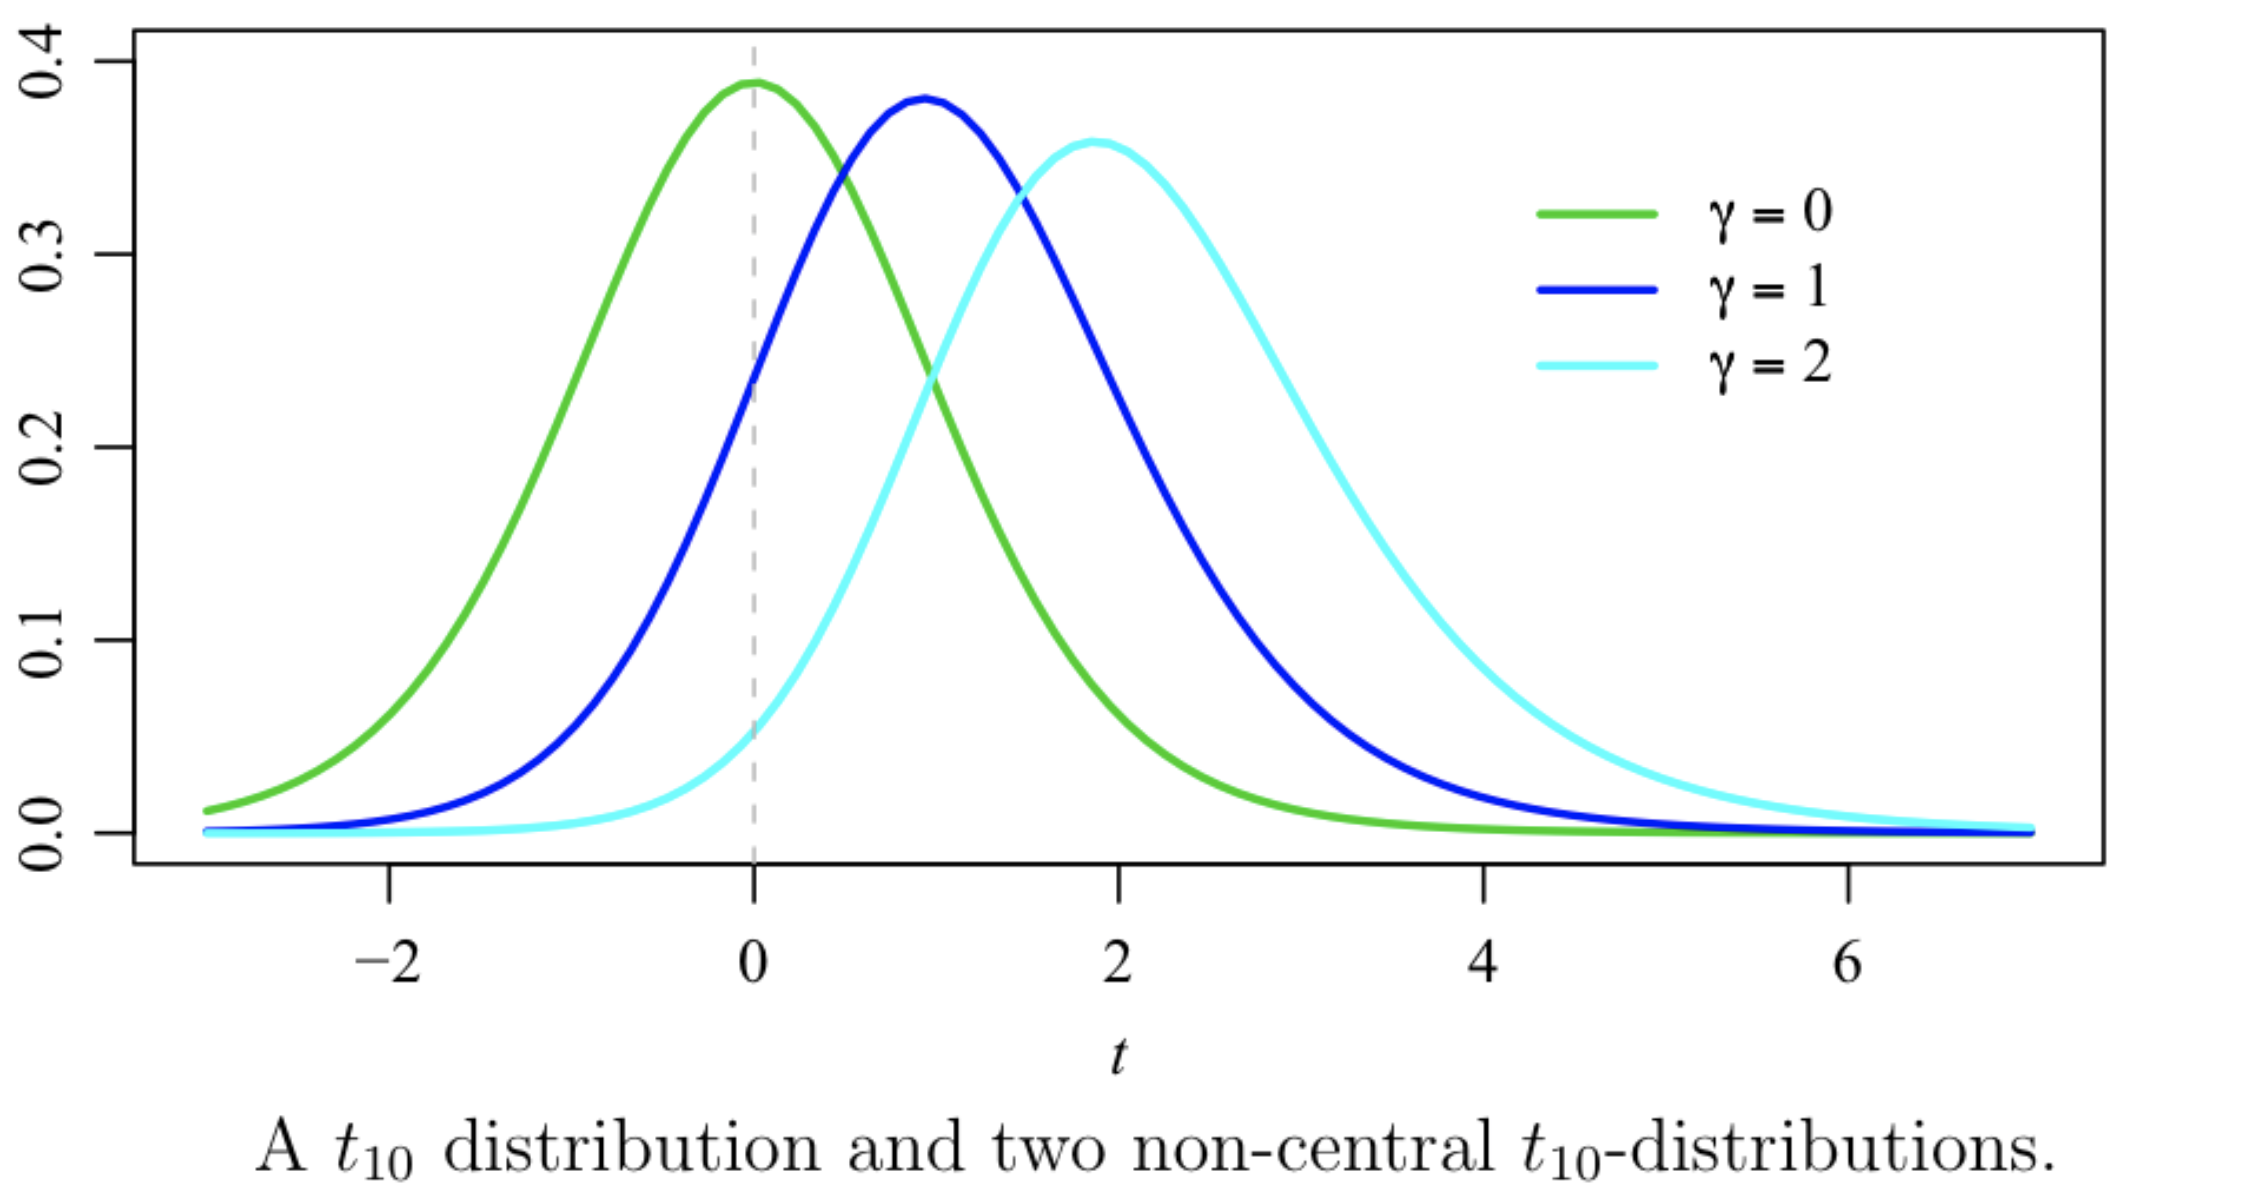
\includegraphics[width=1\textwidth]{fig1.png}
\end{figure}

For a non-central t-distribution:
\begin{itemize}
    \item mean is not zero
    \item distribution is not symmetric
\end{itemize}

\noindent Recall, if data is normally distributed, with common variance:
\[
\bar{Y}_B - \bar{Y}_A \sim \mathcal{N} \left( \delta, \sigma^2 \left( \frac{1}{n_A} + \frac{1}{n_B} \right) \right)
\]
\[
\therefore \frac{\bar{Y}_B - \bar{Y}_A}{\sigma \sqrt{\frac{1}{n_A} + \frac{1}{n_B}}} \sim \mathcal{N} \left( \frac{\delta}{\sigma \sqrt{\frac{1}{n_A} + \frac{1}{n_B}}}, 1 \right)
\]
Also known as \( n_A, n_B \) get large, \( s^2 \approx \sigma^2 \).

$\therefore$ non-central t-distribution statistic will look approximately normal with the above mean and variance.

\subsection*{Computing the Power of a Test}

Recall our level-\(\alpha\) testing procedure using two sample t-test:

\begin{enumerate}
    \item Sample data, compute \( t_{\text{obs}} = t(Y_A, Y_B) \)
    \item Compute p-value: \( P\left( |T_{n_A+n_B-2}| > |t_{\text{obs}}| \right) \)
    \item Reject \( H_0 \) if p-value \(\leq \alpha\).
\end{enumerate}

We have shown,
\[
P(\text{reject } H_0 \mid \mu_B - \mu_A = 0)
\]
\[
= P(\text{p-value} \leq \alpha \mid \mu_B - \mu_A = 0)
\]
\[
= P(|T_{n_A+n_B-2}| \geq t_{1-\alpha/2, n_A + n_B - 2})
\]
\[
= \alpha
\]

Now we want:
\[
P(\text{reject } H_0 \mid \mu_B - \mu_A = \delta)
\]
\[
= P\left( |t(Y_A, Y_B)| > t_c \mid \mu_B - \mu_A = \delta \right)
\]
\[
= P(|T^*| > t_c)
\]
\[
= P(T^* > t_c) + P(T^* < -t_c)
\]
\[
= \left[ 1 - P(T^* < t_c) \right] + P(T^* < -t_c)
\]
\textcolor{red}{Where $T^*$ has a non-central t-distribution with $n_A + n_B - 2$ degrees of freedom and non-centrality parameter}
\[\textcolor{red}{
\Delta ? = \frac{\delta}{\sigma \sqrt{\frac{1}{n_A} + \frac{1}{n_B}}}
}\]

\noindent \textbf{In R:} \\

\begin{lstlisting}
t.crit <- qt( 1 - alpha / 2 , nA + nB - 2 )

t.gamma <- delta / ( sigma * sqrt(1/nA + 1/nB) )

t.power <- 1 - pt( t.crit , nA + nB - 2 , ncp = t.gamma ) +
               pt( -t.crit , nA + nB - 2 , ncp = t.gamma )
\end{lstlisting}

\noindent \textbf{Approximating Power}

\noindent Recall for large \(n_A, n_B\):
\[
t(Y_A, Y_B) \sim \mathcal{N}(\delta, 1)
\]
\[
\Rightarrow \text{power given by } P(|X| > t_c) = [1 - P(X < t_c)] + P(X < -t_c)
\]
\[\textcolor{red}{\text{where } X \sim \mathcal{N}(\delta, 1)}
\]

\begin{lstlisting}
t.norm.power <- 1 - pnorm( t.crit, mean = t.gamma ) + 
                    pnorm( -t.crit, mean = t.gamma )
\end{lstlisting}
    
\subsection*{Sample Size Estimation}
How big should the sample size be if we want to reject
\[
H_0: \mu_B - \mu_A = 0 \quad \text{at} \quad \alpha = 0.05
\]
with true \(\mu_B - \mu_A = 5\) or more?
\vspace{0.5cm}

What we have:
\begin{itemize}
    \item effect size = 5
    \item \(\sigma^2\) unknown, replace with our estimate \(s^2 = 22.24 = \hat\sigma^2\)
\end{itemize}

\noindent Simplify by letting 
\[n_A = n_B = n\]
\[
\Rightarrow \gamma = \frac{\mu_B - \mu_A}{\hat{\sigma} \sqrt{\frac{1}{n_A} + \frac{1}{n_B}}}
\textcolor{red}{\quad (\mu_B - \mu_A \text{ is } \delta )}
\]
\[
= \frac{5}{4.75 \sqrt{\frac{2}{n}}} = 0.75 \sqrt{n}
\]

\noindent What is the probability we reject $H_0$ at level $\alpha$ for a given sample size? \\

\begin{lstlisting}
delta <- 5 ; s2 <- ( (nA-1)*var(yA) + (nB-1)*var(yB) ) / (nA-1+nB-1)

alpha <- 0.05 ; n <- seq(6,30)
    
t.crit <- qt(1-alpha/2, 2*n-2)
    
t.gamma <- delta / sqrt(s2*(1/n+1/n))
    
t.power <- 1 - pt(t.crit, 2*n-2, ncp=t.gamma) + 
            pt(-t.crit, 2*n-2, ncp=t.gamma)

t.normal.power <- 1 - pnorm(t.crit, mean=t.gamma) + 
            pnorm(-t.crit, mean=t.gamma)
\end{lstlisting}
    
\begin{figure}[H]
    \centering
    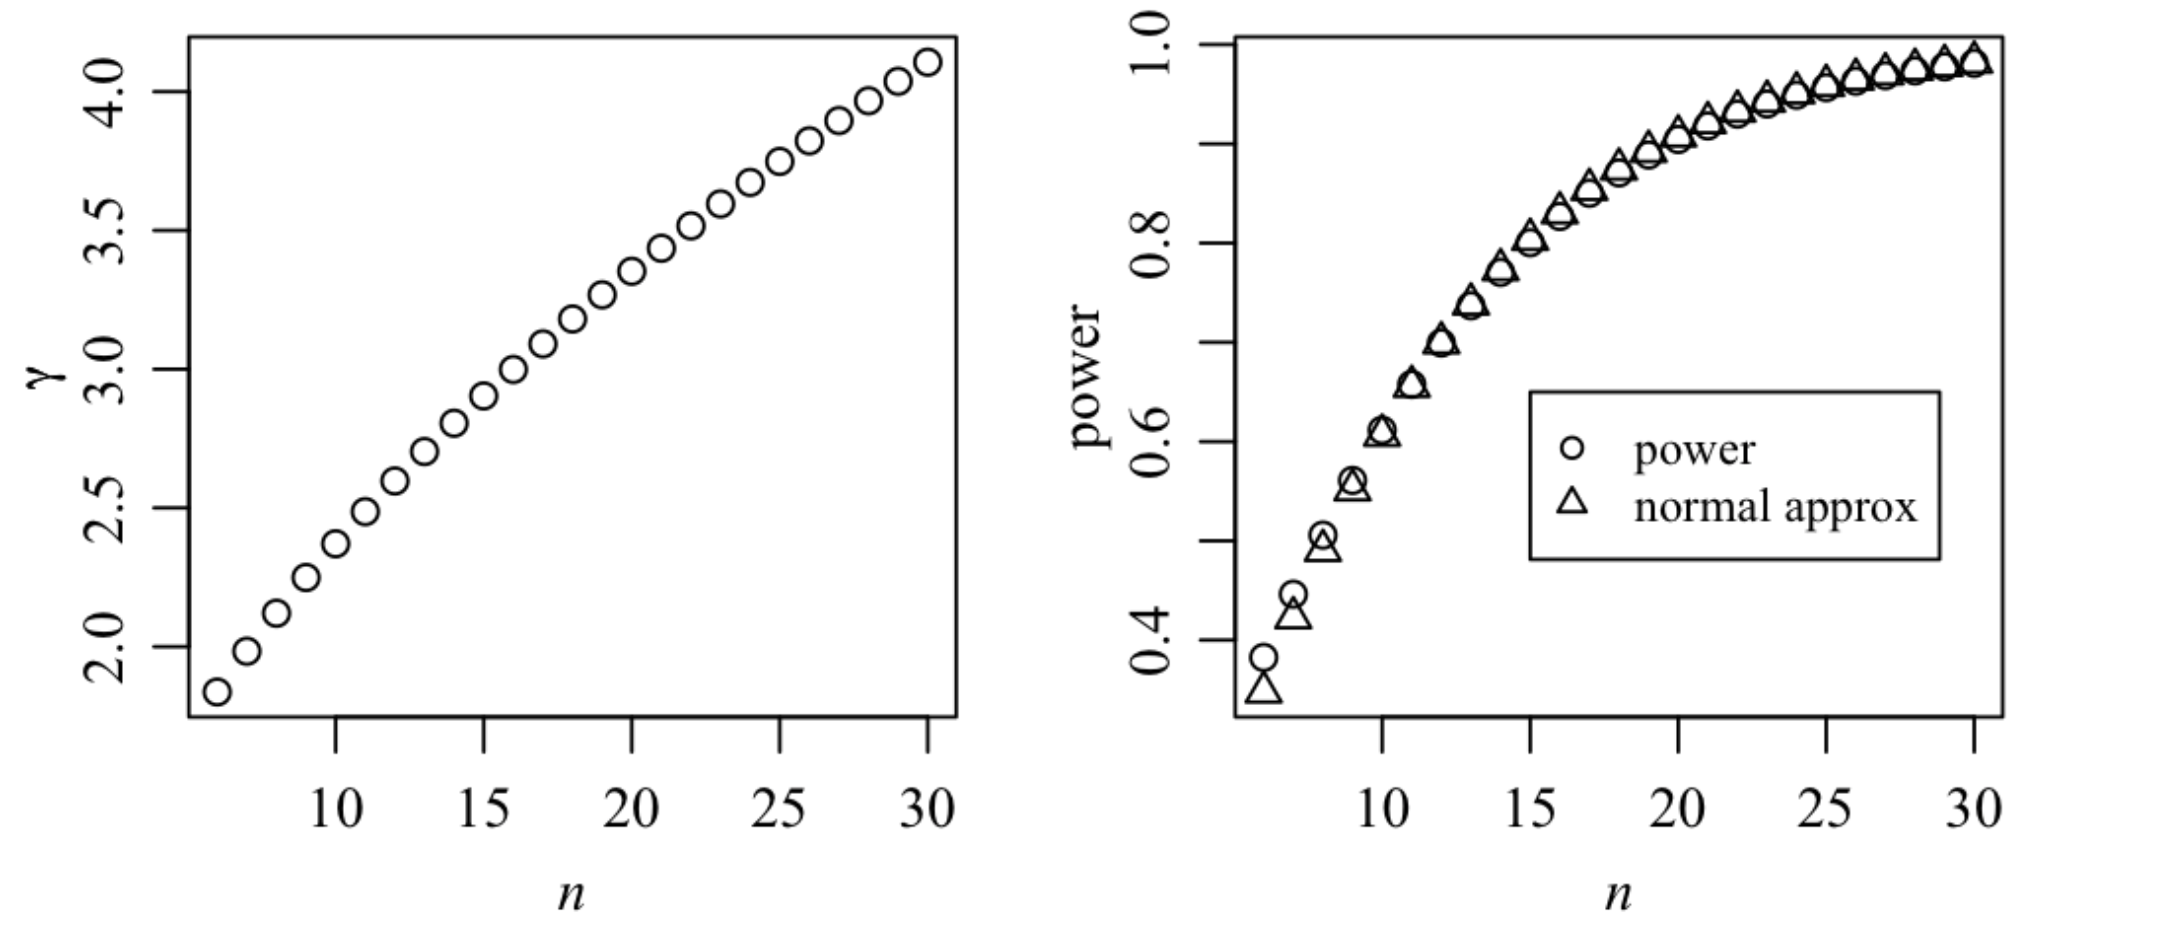
\includegraphics[width=1\textwidth]{fig5.png}
\end{figure}
\noindent To have $80\%$ power, require
\[
n_A = n_B = 15 \quad \text{if true} \quad \mu_B - \mu_A = 5
\]

\subsection*{Increasing Power}

Recall normal approximation to power, for fixed \(\alpha\), power is a function of
\[
\gamma = \frac{\mu_B - \mu_A}{\sigma \sqrt{\frac{1}{n_A} + \frac{1}{n_B}}}
\]

$\therefore$ power is:
\begin{itemize}
    \item increasing in \( |\mu_B - \mu_A| \)
    \item increasing in \(n_A\) and \(n_B\)
    \item decreasing in \(\sigma^2\)
\end{itemize}
\subsection*{Sample size for a Given Precision}

To design a study that will pin down the estimate of \( \mu_B - \mu_A \) to within \(\pm m\) with \(1 - \alpha\) confidence, when \(n_A = n_B = n\), and when \(n\) is large enough so that \(t_{2n-2, 1 - \alpha / 2}\) can be approximated by the critical value from \(\mathcal{N}(0, 1)\) 
\[\text{[e.g. } z = 1.96 \text{ when } \alpha = 0.05]\]
\[
\Rightarrow n = 2 \left[ \frac{Z \sigma}{m} \right]^2
\]

\subsection*{Large-Sample Confidence Interval for \( p \)}

An approximate CI for the population proportion \( p \) is given by:
\[
\hat{p} \pm z^* SE \text{ where } SE = \sqrt{\frac{\hat{p}(1 - \hat{p})}{n}}
\]
\textcolor{red}{\( z^* \) is the critical value corresponding to the desired confidence level $Z_{1-\alpha/2}$ }

\noindent where onfidence levels and corresponding \( z^* \) values:
\[
\begin{array}{c|c c c}
\text{Confidence Level} & 90\% & 95\% & 99\% \\
\hline
z^* & 1.645 & 1.960 & 2.576 \\
\end{array}
\]

\noindent \textbf{Remark:} The exact SE should be \( \sqrt{\frac{p(1 - p)}{n}} \), but the unknown \( p \) is replaced with the estimate \( \hat{p} \). This large-sample CI is not very accurate, meaning the actual confidence level often falls below the nominal level.

\subsection*{Example: Side Effects of Pain Relievers (1)}

Arthritis is a painful, chronic inflammation of the joints, so many arthritis patients rely on pain relievers, like Ibuprofen. However, Ibuprofen may induce side effects (like dizziness, muscle cramp, allergy, or even seizure) on some patients.

\noindent A study interviewed 440 arthritis patients taking Ibuprofen, and found 23 had experienced side effects. Suppose the 440 patients is a Simple Random Sample (SRS) from the population of arthritis patients taking Ibuprofen.

\noindent Find a 90\% confidence interval for the population proportion \( p \) of arthritis patients who suffer some adverse symptoms.
\vspace{0.5cm}

The sample proportion is \(\hat{p} = \frac{23}{440} \approx 0.052\).

The \(z^*\) for a 90\% CI is 1.645. So a 90\%-CI for \(p\) is
\[
\hat{p} \pm z^* \sqrt{\frac{\hat{p}(1 - \hat{p})}{n}} \approx 0.052 \pm 1.645 \sqrt{\frac{0.052 \times (1 - 0.052)}{440}}
\]
\[
\approx 0.052 \pm 0.017 = (0.035, 0.069)
\]

Conclusion: With a 90\% confidence, between 3.5\% and 6.9\% of arthritis patients taking this pain medication experience some adverse symptoms.

\subsection*{Choosing a Sample Size}

How large the sample size \(n\) need to be to make the margin of error of a CI \(\leq m\)?
\[
\text{margin of error} = z^* \sqrt{\frac{\hat{p}(1-\hat{p})}{n}} \leq m 
\quad \Rightarrow \quad n \geq \left(\frac{z^*}{m}\right)^2 \hat{p}(1-\hat{p})
\]

\noindent \textcolor{blue}{But} \(\hat{p}\) is UNKNOWN before we get the data. Need to make a guess for \(p^*\). How to choose \(p^*\)?
\begin{enumerate}
    \item Conduct a small pilot study, or use prior studies or knowledge to get a range for possible values of \(p\). Choose the bound that is closer to 0.5. E.g., if possible range of \(p\) is [0.1, 0.2], choose \(p^* = 0.2\). 
    If the possible range of \(p\) is [0.85, 0.95], choose \(p^* = 0.85\).
    \item The most \textbf{conservative} approach is to choose \(p^* = 0.5\) since the margin of error is the largest when \(\hat{p} = 0.5\).
\end{enumerate}

\subsection*{Example – Sample Size Calculation for a Proportion}

A 1993 survey reported that 72.1\% of freshmen responding to a national survey were attending the college of their first choice. Suppose that \(n = 500\) students responded to the survey.

\begin{enumerate}
    \item Find a 95\% Confidence Interval (CI) for the proportion \(p\) of college freshmen attending their first choice college.
    \item Suppose that given the CI, we want to conduct a survey which has a margin of error of 1\% (i.e., \(m = 0.01\)) with 95\% confidence. How many people should we interview?
\end{enumerate}

The two-sided 95\% confidence interval is:
\[
\hat{p} \pm z^* \sqrt{\frac{\hat{p}(1 - \hat{p})}{n}} = 0.721 \pm 1.96 \sqrt{\frac{0.721(1 - 0.721)}{500}}
\]
\[
= (0.682, 0.760)
\]

We have good reason to believe \(p\) is in that range. For a sample size calculation, we choose the \(p\) closest to 0.5, that is \(p = 0.682\).
\[
\left( \frac{z^*}{m} \right)^2 p(1 - p) = \left( \frac{1.96}{0.01} \right)^2 \times 0.682(1 - 0.682) \approx 8331.51
\]

The required sample size is 8332. We need a much larger sample size than the original study because we want a smaller margin of error.

\underline{Remark.} Recall that for confidence intervals, we use
\[
SE = \sqrt{\frac{\hat{p}(1 - \hat{p})}{n}}
\]

but for hypothesis testing we use
\[
SE = \sqrt{\frac{p_0 (1 - p_0)}{n}}.
\]

\noindent \textbf{Why?}
\begin{itemize}
    \item Recall by CLT when \(n\) is large, \(\hat{p} \overset{\cdot}{\sim} N(p, \sqrt{\frac{p(1 - p)}{n}})\)
    \item When constructing CIs for \(p\), \(p\) is unknown, so we estimate \(\sqrt{\frac{p(1 - p)}{n}}\) by \(\sqrt{\frac{\hat{p}(1 - \hat{p})}{n}}\)
    \item Under \(H_0: p = p_0\), \(p\) is known to be \(p_0\). There is no need to estimate \(p\), and the \(\sqrt{\frac{p(1 - p)}{n}}\) is simply \(\sqrt{\frac{p_0(1 - p_0)}{n}}\).
\end{itemize}

\subsection*{Large Sample Confidence Intervals for \( p_1 - p_2 \)}

When \( n_1 \) and \( n_2 \) are both large, 
\[
\hat{p}_1 - \hat{p}_2 \overset{\cdot}{\sim} N \left( p_1 - p_2, \sqrt{\frac{p_1(1 - p_1)}{n_1} + \frac{p_2(1 - p_2)}{n_2}} \right)
\]
An approximate \( (1 - \alpha)100\%\) confidence interval for \( p_1 - p_2 \) is 
\[
\text{estimate} \pm z^* \text{SE}
\]
where 
\[
\text{estimate} = \hat{p}_1 - \hat{p}_2, \quad \text{SE} = \sqrt{\frac{\hat{p}_1(1 - \hat{p}_1)}{n_1} + \frac{\hat{p}_2(1 - \hat{p}_2)}{n_2}}
\]
Use this method only when the number of successes and the number of failures in both samples are at least 10, i.e., 
\[
n_1 \hat{p}_1, \quad n_1(1 - \hat{p}_1), \quad n_2 \hat{p}_2, \quad n_2(1 - \hat{p}_2) \quad \text{all} \geq 10.
\]

\subsection*{Example: Aspirin and Heart Attacks (1)}

The Physicians' Health Study was a 5-year randomized study published testing whether regular intake of aspirin reduces mortality from cardiovascular disease\footnote{Source: Preliminary Report: Findings from the Aspirin Component of the Ongoing Physicians' Health Study. New Engl. J. Med., 318: 262-64, 1988.}.

\begin{itemize}
    \item Participants were male physicians 40-84 years old in 1982 with no prior history of heart attack, stroke, and cancer, no current liver or renal disease, no contraindication of aspirin, no current use of aspirin.
    \item Every other day, the male physicians participating in the study took either one aspirin tablet or a placebo.
    \item Response: whether the participant had a heart attack (including fatal or non-fatal) during the 5-year period.
\end{itemize}

\textbf{Result:}
\[
\begin{array}{c c c c c }
& \multicolumn{2}{c}{\text{Heart Attack?}} & & \\
\cline{2-3}
\text{Group} & \text{Yes} & \text{No} & \text{Sample Size} & \text{ }\\
\hline
\text{Placebo} & 189 & 10845 & 11034 & \quad \Rightarrow \hat{p}_1 = \frac{189}{11034} \approx 0.0171 \\
\text{Aspirin} & 104 & 10933 & 11037 & \quad \Rightarrow \hat{p}_2 = \frac{104}{11037} \approx 0.0094 \\
\hline
\end{array}
\]

The \(z^*\) for a 99\% CI is 2.58, so the 99\% CI for \(p_1 - p_2\) is
\[
\hat{p}_1 - \hat{p}_2 \pm z^* \sqrt{\frac{\hat{p}_1(1 - \hat{p}_1)}{n_1} + \frac{\hat{p}_2(1 - \hat{p}_2)}{n_2}}
\]
\[
= 0.0171 - 0.0094 \pm 2.58 \sqrt{\frac{0.0171(1 - 0.0171)}{11034} + \frac{0.0094(1 - 0.0094)}{11037}}
\]
\[
= 0.0077 \pm 0.0040 = (0.0037, 0.0117)
\]

\textbf{Conclusion:}
\begin{itemize}
    \item As the 99\% CI does not contain 0, the incidence rate of heart attack was significantly lower in the aspirin group than in the placebo group \(\textcolor{red}{\text{(at } \alpha = 0.01\text{)}}\).
    \item Can we claim that taking aspirin every other day is effective in reducing the chance of heart attack? 
    \textcolor{orange}{\textbf{Yes, because it was a randomized, double-blind, placebo-controlled experiment.}}
\end{itemize}

\subsection*{Summary: Standard Errors}

\hspace{-1.5cm}
\begin{tabular}{c|c|c}
 & \textbf{One Sample} & \textbf{Two Samples} \\
\hline
\textbf{Mean} & $\dfrac{s}{\sqrt{n}}$ & $\sqrt{\dfrac{s_1^2}{n_1} + \dfrac{s_2^2}{n_2}} \quad \text{if} \quad \sigma_1 \neq \sigma_2$ \\[10pt]
 & & $s_p \sqrt{\dfrac{1}{n_1} + \dfrac{1}{n_2}} \text{ if } \sigma_1 = \sigma_2 \text{ where } s_p = \sqrt{\dfrac{(n_1-1)s_1^2 + (n_2-1)s_2^2}{n_1+n_2-2}}$ \\[10pt]
\hline
\textbf{proportion} & $\sqrt{\dfrac{\hat{p}(1-\hat{p})}{n}}$ & $\sqrt{\dfrac{\hat{p}_1(1-\hat{p}_1)}{n_1} + \dfrac{\hat{p}_2(1-\hat{p}_2)}{n_2}}$ \\[10pt]
\textbf{(CIs)} &  & \\[10pt]
\hline
\textbf{proportion} & $H_0: p = p_0$ & $H_0: p_1 = p_2 \quad \sqrt{\hat{p}(1-\hat{p})\left(\dfrac{1}{n_1} + \dfrac{1}{n_2}\right)} \quad \text{where} \quad \hat{p} = \dfrac{X_1+X_2}{n_1+n_2}$ \\[10pt]
\textbf{(Tests)} & $\sqrt{\dfrac{p_0(1-p_0)}{n}}$ & \\[10pt]
\end{tabular}
\vspace{0.5cm}

\textbf{Use the ones from CIs as part of margin of error calculations.}

\section*{Sample Size for Comparing Two Proportions}

Using the idea of a given precision
\[
m = Z_{1-\alpha/2} \sqrt{\frac{\hat{p}_1(1 - \hat{p}_1)}{n_1} + \frac{\hat{p}_2(1 - \hat{p}_2)}{n_2}}
\]

\noindent For fixed \(n_1 = n_2 = n\), CIs for the independent comparing proportions has maximum width when \(p_1 = p_2 = 0.5\).

\noindent \textbf{Why?}

Recall
\[
\text{var}(\hat{p}_1 - \hat{p}_2) = \frac{\hat{p}_1(1 - \hat{p}_1)}{n_1} + \frac{\hat{p}_2(1 - \hat{p}_2)}{n_2}
\]

When \(p_1 = p_2 = p\) and \(n_1 = n_2 = n\)

\[
\Rightarrow \frac{\hat{p}(1 - \hat{p})}{n} + \frac{\hat{p}(1 - \hat{p})}{n}
\]

\[
= 2 \frac{\hat{p}(1 - \hat{p})}{n}
\]
\[
\textcolor{red}{\text{maximized when } \hat{p} = 0.5}
\]

When this is used, further simplification:

\[
\Rightarrow 2 \cdot \frac{0.25}{n} = \frac{1}{2n}
\]

Using $\alpha = 0.05 \left( Z^* = 1.96 \right)$ , worst case margin of error is:

\[
m = 1.96 \sqrt{\frac{1}{2n}}
\]

\[
\Rightarrow n = \frac{1.92}{m^2}
\]

This gives a formula for the number of subjects in each group \(n\) to obtain a given margin of error \(m\).







\end{document}